\documentclass[a4paper,12pt]{article}
\usepackage{blindtext}
\usepackage[utf8]{inputenc}
\usepackage{graphicx}
\usepackage{enumitem}

\begin{document}
\begin{titlepage}
\center

\textsc{\LARGE Architectural Requirements}\\[1.5cm]
\textsc{\Large Project: Traffic Camera Image Analysis}\\[1.5cm]
\textsc{\large Client: DPSS, CSIR}\\[0.5cm]
\textsc{\large Team: Quadcore Productions}\\[0.5cm]

\begin{minipage}{0.4\textwidth}
\begin{flushleft} \large
\emph{Author(s):}\\
Mpho \textsc{Baloyi}\\
Hlengekile \textsc{Jita}\\
Mayimela \textsc{Moses}\\
Mbhele \textsc{Themba}\\
\end{flushleft}
\end{minipage}
~
\begin{minipage}{0.4\textwidth}
\begin{flushright} \large
\emph{Student number(s):} \\
14133670\\ % Student number
14077893\\
14019702\\
14007950\\
\end{flushright}
\end{minipage}\\

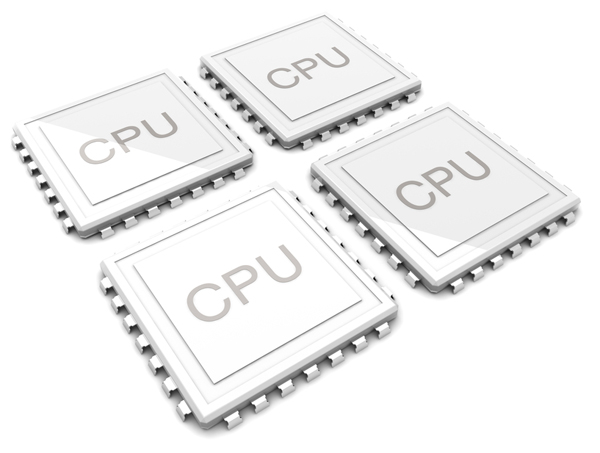
\includegraphics[width=\textwidth]{2012-quad-core-phones.jpg}

{\large University of Pretoria, Department of Computer Science}\\

{\large 27 May 2016}\\[3cm]

\vfil

\end{titlepage}

\newpage
\tableofcontents
\newpage
\section{Introduction}
This document describes the architectural requirements of the Traffic Camera Image Analysis System. The target system will run on a web server  and be accessed by users on an Android Application which will provide the users with the necessary functionality to access real-time traffic information that assists them with things such as avoiding traffic and choosing the best alternative routes.

In this specification we will cover the architectural scope of the system, the quality requirements, integration and access channel requirements and architectural constraints. In addition we will describe the software architecture we will use by describing the architectural patterns and tactics we will use as well as which frameworks and technologies will be used to achieve them.
\section{Vision}
For this project we aim to achieve a system that makes use of images obtained from highway cameras to provide users with up-to-date real-time traffic information. The system should simplify the user's travels by providing traffic information and notifying them before they depart of traffic conditions, calculating arrival times based on traffic conditions and help them select the most suitable route for their trips using the traffic information and additional metrics. Our vision for the target system is that it should be reliable and perform relatively quickly, both for user satisfaction and in order to be the an up-to-date traffic information system.
\section{Background}
As a commuter, traffic is something that is a part of everyday life, and it is not one of the more pleasurable aspects of life. Already there is software in place that assists us in dealing with this problem, such as Google Maps. This software uses the crowd-sourcing of GPS data in order to provide their up-to-date traffic information.

In our system,we want to take an image analysis approach to solve the same problem. We will make use of the publicly available SANRAL highway cameras to get images which can be found on https://www.i-traffic.co.za/traffic/cameras.aspx. Processing these images we will perform image analysis and determine the traffic conditions in the area of a camera. Using this information we will be able to generate information pertaining to user specified routes in order to provide the information necessary to help them avoid traffic and choose the most suitable routes in order to do so.

\section{Architectural Requirements}
\subsection{Architectural Scope}

\subsection{Quality Requirements}
\subsubsection{Usability}
Usability is the key component of the system because user satisfaction is a high priority for this system because it aims to alleviate a problem that individuals experience daily. The aim is to create that is easy to understand and thus, easy to learn how to us. \\
\textbf{How to achieve usability}
\begin{itemize}
\item The interface of the mobile application will be designed in an intuitive manner meaning that it will be easy to navigate and easy to understand.It will include buttons and other methods of interaction for which their functionality is self explanatory.
\item The interface will only have what is required and nothing more to ensure that it is not cluttered and does not cause confusion.
\item Usability tests will be conducted to ensure the successful implementation of a user friendly application.
\end{itemize}
\subsubsection{Scalability}
Scalability refers to a systems ability to handle a heavy workload. We have identified this as an important aspect of the system because a report will have to be provided at a very fast speed because traffic changes rapidly and we need to keep up with the traffic updates. Also, multiple users will be making use of the system at the same time and they all need to be catered to at the same levels of performance. \\
\textbf{How to achieve usability}
\begin{itemize}
\item To improve the performance of the system, reports will only be generated when it is necessary to do so. To elaborate on this, the website from which we will be getting the images from updates its images at one minute intervals so between that period, we will not attempt to grab new images but will make use of the images that were grabbed at the previous interval. In this way, no unnecessary processing takes place.
\item We will not generate a new report if it is not necessary to do so. If we generate a report for one user and another user requests a report for the exact same route when it is not time to update the images, we will use the same report that was generated for the first user. We will do this by implementing a cache server to store route reports.  
\end{itemize}
\subsubsection{Maintainability}
The components of the system need to implemented in a manner that makes it easy for them to be updated or replaced.\\
\textbf{How to achieve maintainability}
\begin{itemize}
\item Maintainability will be achieved by writing loosely coupled code.
\end{itemize}
\subsubsection{Reliability}
Reliability is of utmost importance because a lot of people will be using the application, especially at traffic peak hours thus the system has to get the job done and it should do it effectively so that users get the best service possible. \\
\textbf{How to achieve reliability} \\
\begin{itemize}
\item The main focus will be placed on the prevention of faults. This will be done by testing the system extensively and working towards fixing any fault that is encountered.
\end{itemize}
\subsection{Integration and Access Channel Requirements}
\subsection{Architectural Constraints}
\subsubsection{Technologies}
\begin{itemize}
\item Python: Python will be used to implement the web server of the system which will perform the necessary processing of data and after completion, the server will send the data to the mobile application via Google Cloud Messaging.
\item OpenCv: OpenCv is an image processing library that the server will make use of to process the traffic images from SANRAL.
\item Android Studio: Android Studio will be used to design a mobile application on which traffic reports will be displayed.
\end{itemize}
\section{Initial Software Architecture Design}
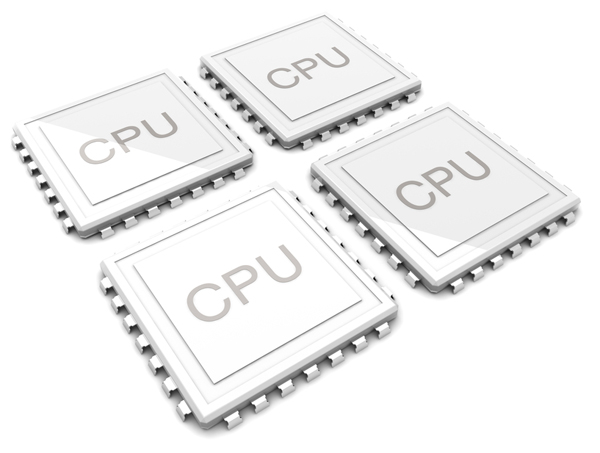
\includegraphics[width=\textwidth]{2012-quad-core-phones.jpg}
\end{document}